\documentclass[12pt]{article}

\usepackage[letterpaper,margin=1in]{geometry}
\linespread{1.6} % double spacing
\raggedright
\setlength{\parskip}{1em}

\usepackage{fontspec}
\usepackage[utf8]{inputenc}
\usepackage{microtype}

% \usepackage[hyphens]{url}
% \usepackage[hidelinks]{hyperref}
% \usepackage{sectsty}
\usepackage [english]{babel}
\usepackage [autostyle, english = american]{csquotes}
\MakeOuterQuote{"}

% \usepackage[backend=biber,style=ieee]{biblatex}
% \addbibresource{sources.bib}

\usepackage{graphicx}
\usepackage{wrapfig}
\usepackage{float}

\setromanfont{Source Serif Pro}
\setsansfont{Iosevka Type}
\setmonofont{Iosevka Term}

% \usepackage[familydefault,light]{chivo}

\title{\texttt{{\Huge GT ORG ANALYTICS} \linebreak {\normalsize Final Report, CS 4365 Spring 2017}}}
\author{\texttt{{\normalsize Daniel Theriault}}}
\date{\texttt{{\normalsize \today}}}

\begin{document}
\maketitle \pagebreak
% \tableofcontents \pagebreak


\section*{Introduction}

My project addresses the need of student organizations for tools to analyze their event attendance data by generating reports on data stored with the OrgSync organization management platform.

This final report document includes:
\begin{itemize}
    \item An overview of my project implementation, with a supporting rationale for important choices.
    \item Usage examples illustrating the use of the command-line interface, and some likely combinations of options.
    \item My current vision of future development for this program
    \item A brief reflection and conclusion of this project
\end{itemize}


\section*{Completed Works}
The deliverable version of GT Org Analytics contains two main components: a data-processing portion, which parses information taken from the GT OrgSync platform and stores it in a relational database, and a report-generating portion, which uses this data to build user-ready pdf reports.
Each of these reports focuses on a specified set of events hosted by the organization, or makes a comparison between two such sets.
My initial proposal did include a wider set of distinct analyses; however, during implementation I realized that a smaller, more flexible set of functions could provide the same information to users.
I opted to produce a tool that is more flexible, extensible, and maintainable while covering a similar feature set.


\section*{Project Architecture}

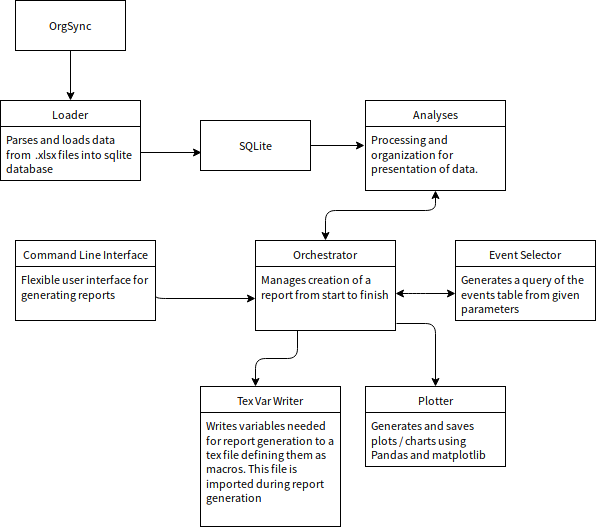
\includegraphics[width=6in]{./media/architecture.png}
\pagebreak

\textbf{Project Directory Layout }
\begin{verbatim}
    GT Org Analytics
    ├── analyses.py
    ├── cli.py
    ├── Data
    │   ├── Community Dinner Participation1.xlsx
    │   ├── ....
    │   └── Theology of the Body Participation.xlsx
    ├── dbinit.py
    ├── events.db
    ├── eventselector.py
    ├── GTCSO.db
    ├── loader.py
    ├── orchestrator.py
    ├── plotter.py
    ├── Reports
    │   ├── comparison.pdf
    │   ├── standard.pdf
    │   └── texput.log
    ├── Templates
    │   ├── comparison.tex
    │   └── standard.tex
    ├── texvar.py
    └── .working
        ├── vars.tex
        └── ... [image files]
\end{verbatim}
\pagebreak

\subsection*{Data Organization}

The original hope for this portion of the project was to pull data directly from the Georgia Tech OrgSync instance via their API.
This goal was not attainable; the OrgSync API does not have permissions management, so all its users have access to all data on the instance.
Georgia Tech, out of concern for privacy and security, does not grant students access to this API.
OrgSync is, however, working on a new version of the API.
Some student organizations have even reverse-engineered this unstable API to support their needs.
I did not consider this a suitable choice for my project, in light of the difficulty of uncovering API details and high risk of breaking changes.
I instead downloaded the individual participation data files from OrgSync event pages, and parsed these files.

This solution is non-ideal, and will be replaced when the new API becomes official.
In order to make future refactoring manageable, this component of the project is very loosely coupled with the report generator; aside from the shared SQLite database, the only interaction between the two components is a single global variable defined in loader.py.

There are two modules in this component:

\texttt{\textbf{dbinit.py}} performs the initial set-up of a SQLite database. 
If an argument is specified, it will attempt to load files from a directory of that name into the database by calling loader.py.
This file contains the \texttt{SQL CREATE TABLE} statements.

\texttt{\textbf{loader.py}} is responsible for parsing the .xlsx files and inserting this information into the database.
This module made use of the excellent \texttt{xlrd} package, which made reading information from .xlsx files very simple.

\subsection*{Report Generator}
Report generation functionality made up the bulk of the work on this project.
I choose to focus on this functionality because it increases the impact of the analytical tooling; pdf-formatted reports are highly portable, and can be shared well beyond the computer running this software.
Report generation uses the LaTeX typesetting language.
It's an older tool, but it allowed for the programmatic generation of well-formatted and attractive pdf reports.
Preparing report templates was also greatly simplified by LaTeX's strong ecosystem of plugins and online community of users.

This component of the project contains a number of individual modules:

The \texttt{\textbf{orchestrator.py}} module controls the overall flow of report generation.
It can orchestrate the generation of two distinct report types: "Standard Reports" and "Comparison Reports".
The methods to generate these reports are distinct, but follow a similar flow and call upon the same set of supporting classes.
The orchestrator takes in any or all of the following as arguments: a list of event names, a list of dates, a range of dates, and special options.

The event names, list of dates, and range of dates are passed to \texttt{\textbf{eventselector.py}}, which will generate a SQL query to select the corresponding events.
This query is returned to orchestrator, and run to produce the events list.
Another method in the module is used to generate a human-readable name for this events list, which is shown at the top of every report.

The orchestrator then uses \texttt{\textbf{analyses.py}} to gather and organize useful information about the events in the list.
Some additional organization and processing of this data occurs in the orchestrator.
Other data has its final processing stage in \texttt{\textbf{plotter.py}}, which uses the \texttt{Pandas} data visualization library, and \texttt{matplotlib} to generate attractive graphical displays; for now, this means bar charts, graphs, and Venn diagrams.
The filenames of these generated images are recorded, alongside all other data used in the eventual report, inside a python dictionary.

This dictionary is passed to \texttt{\textbf{texvar.py}}.
This file writes to vars.tex, defining all entries of the dictionary as LaTeX macros; the key becomes the macro name, and the value becomes its content.
An \verb'\include' statement inside each template brings this variable content into the pdf generation process.

Upon return, the orchestrator carries out the actual compilation of the report from source files, cleans up files and connections, and completes its execution.

\subsection*{Interface}
Due to time pressures and design difficulties, GT Org Analytics is accessed via a command-line interface rather than a graphical interface.
This interface is implemented in \texttt{\textbf{cli.py}}, which uses the \texttt{argparse} python library to implement a clean way of using this program.
The help text explains the basic usage:

\begin{verbatim}
    $ organ -h
    usage: organ [-h] [--emails] [--zathura] [--okular] [--verbose]
              [--names [NAMES [NAMES ...]]] [--dates [DATES [DATES ...]]]
              [--start [STARTDATE]] [--end [ENDDATE]]
              {vs} ...

    Org Analytics report generator.

    positional arguments:
      {vs}

    optional arguments:
      -h, --help            show this help message and exit
      --emails              Enable generation of email lists.
      --zathura             Show report in zathura pdf reader.
      --okular              Show report in kde's okular pdf reader.
      --verbose, -v         Show more information during report generation.
      --names [NAMES [NAMES ...]], -n [NAMES [NAMES ...]]
                            Names of events to include in report
      --dates [DATES [DATES ...]], -d [DATES [DATES ...]]
                            ISO 8601 formatted dates of events to include in
                            report
      --start [STARTDATE], -s [STARTDATE]
                            ISO 8601 formatted date starting a date-range
                            selection for event inclusion
      --end [ENDDATE], -e [ENDDATE]
                            ISO 8601 formatted date terminating a date-range
                            selection for event inclusion, defaults to today.
\end{verbatim}

The positional argument \textbf{vs} is an optional subcommand, which itself can take in names, dates, and start/end dates.
The event groups passed by the main command and the vs subcommand are then compared.
Usage examples, alongside their outputs, are included in the next section.

Please note that 'organ' is an alias on my machine, not a proper binding-point to the program.
To use these commands on another machine, run \texttt{python3 cli.py [ARGS]} from the project directory.


\section*{Usage Examples}
Generate a report on all events in the database:

\texttt{ \$ organ}
\begin{figure}[H]
    \centering
    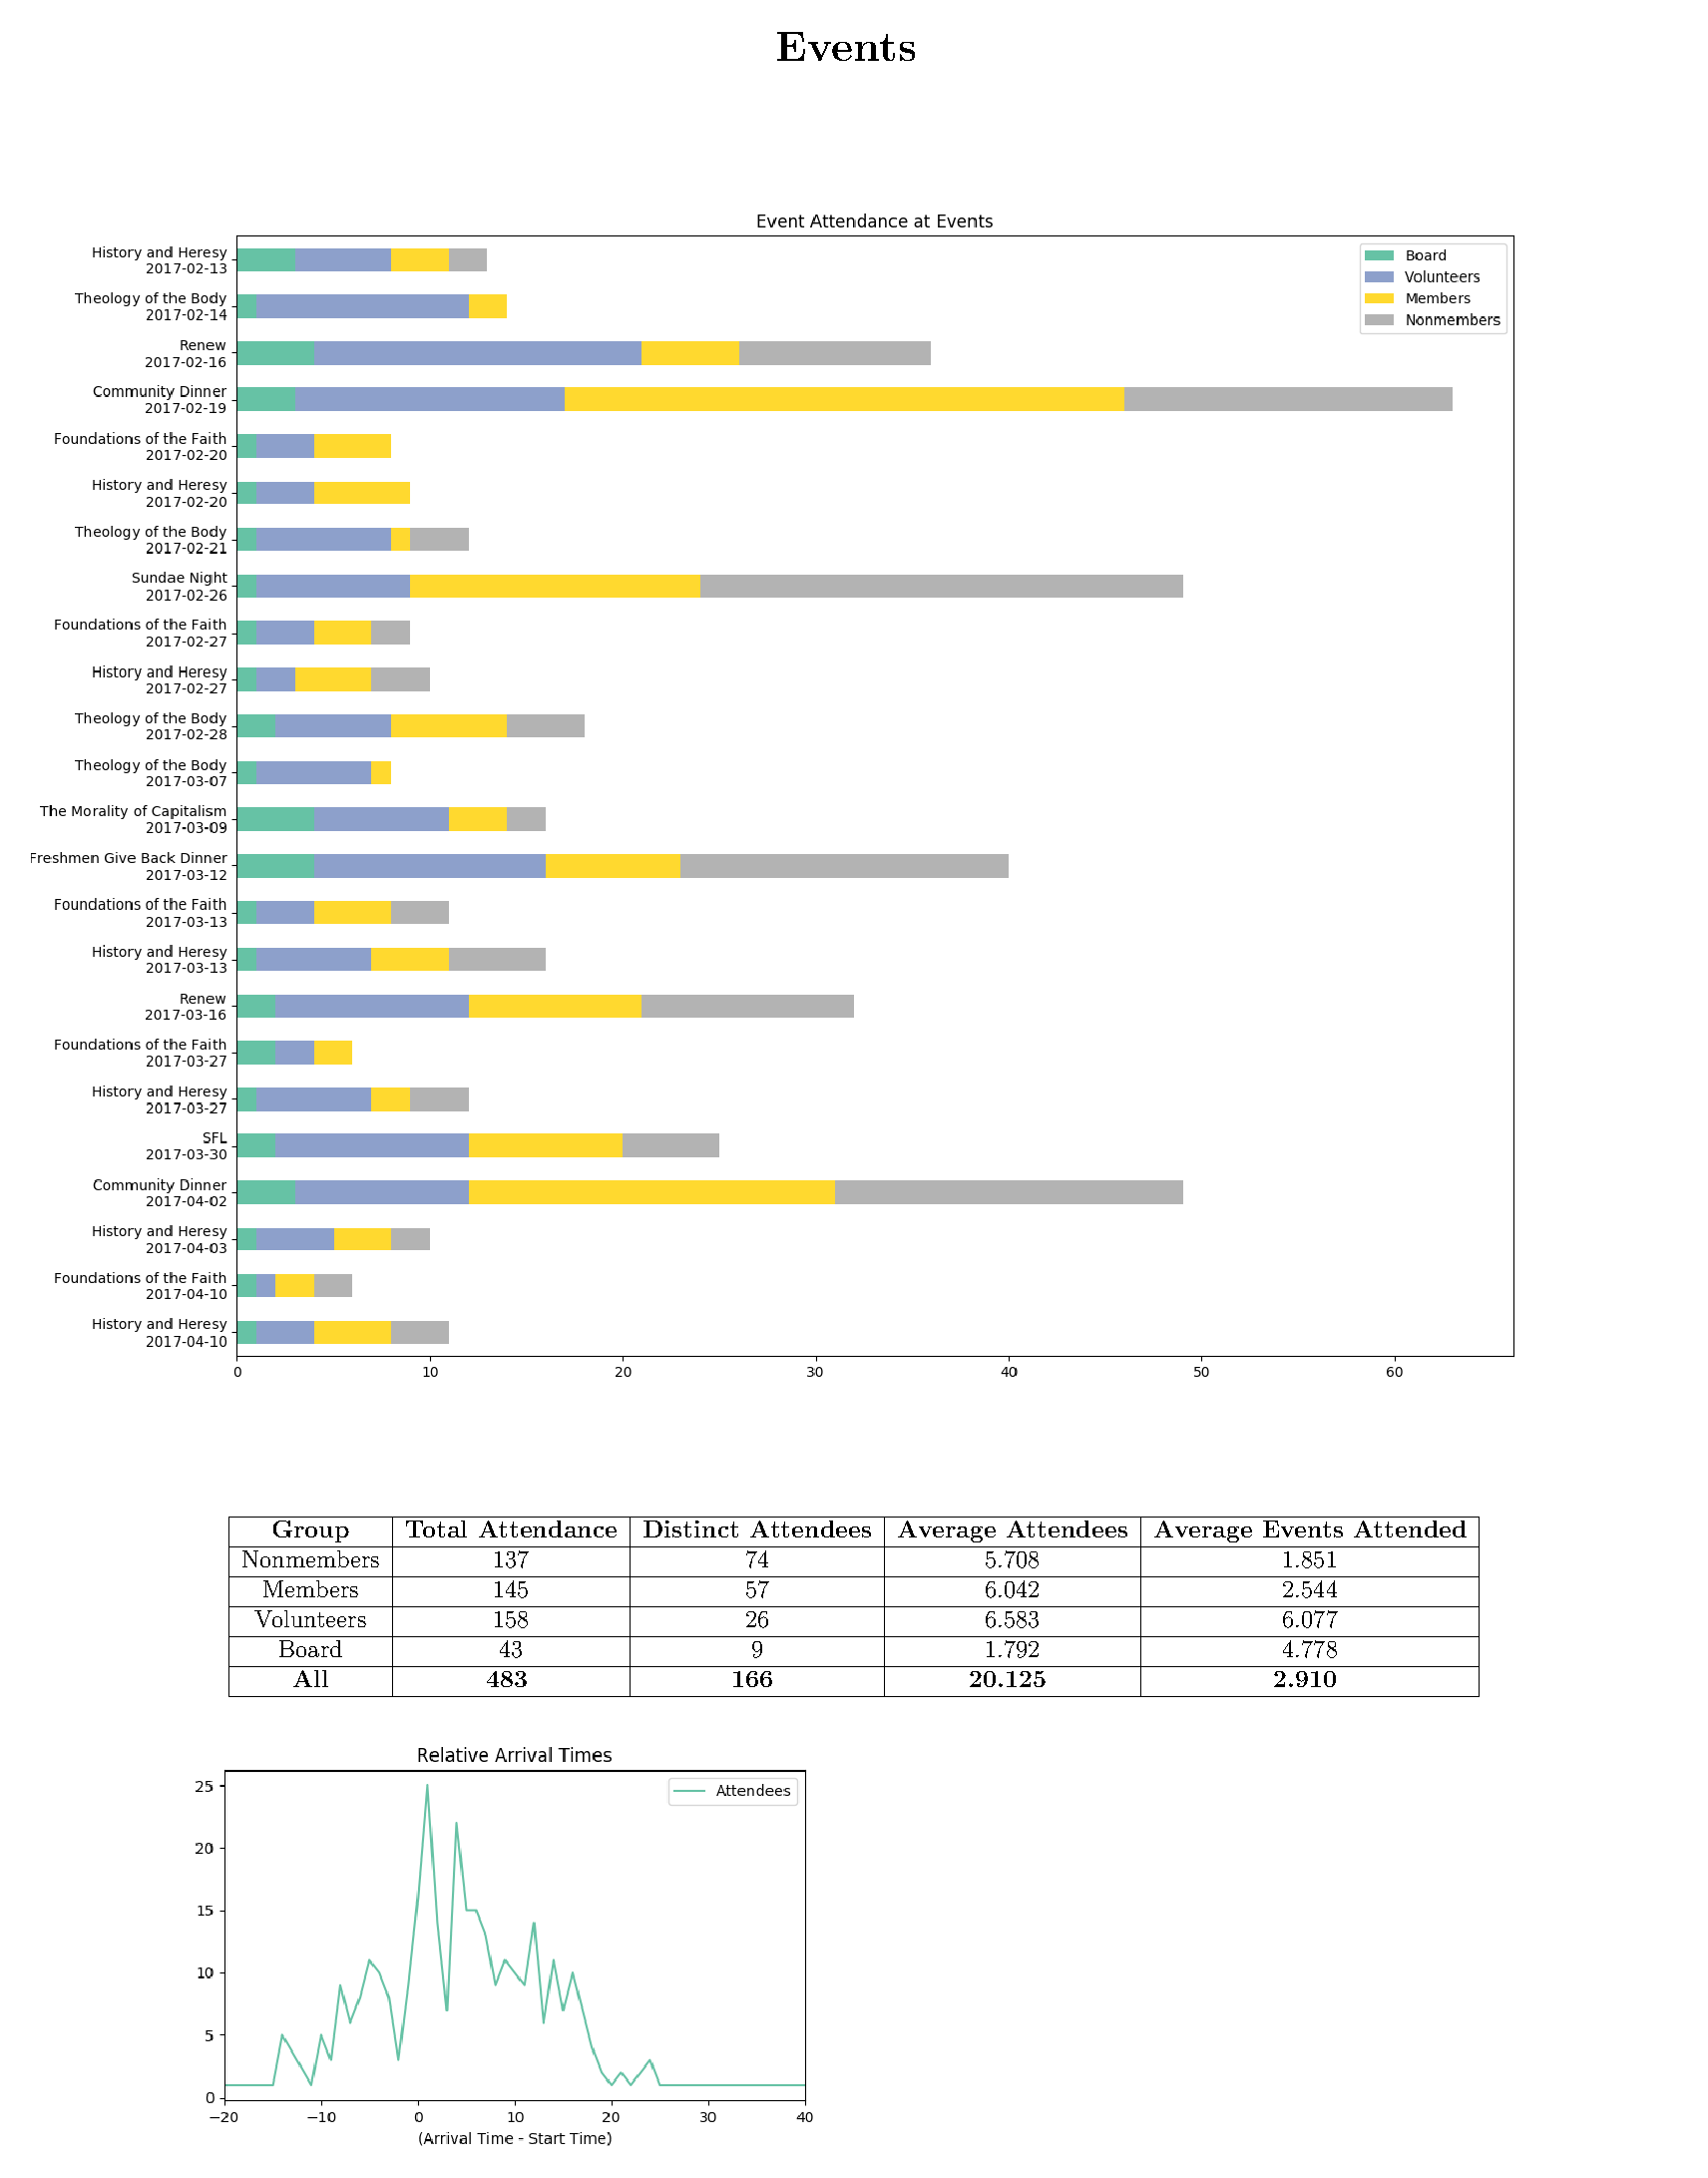
\includegraphics[width=5.3in]{./media/all.pdf}
\end{figure}
\pagebreak
 
Generate a report on all events named 'Renew':

\texttt{ \$ organ --names Renew}
\begin{figure}[H]
    \centering
    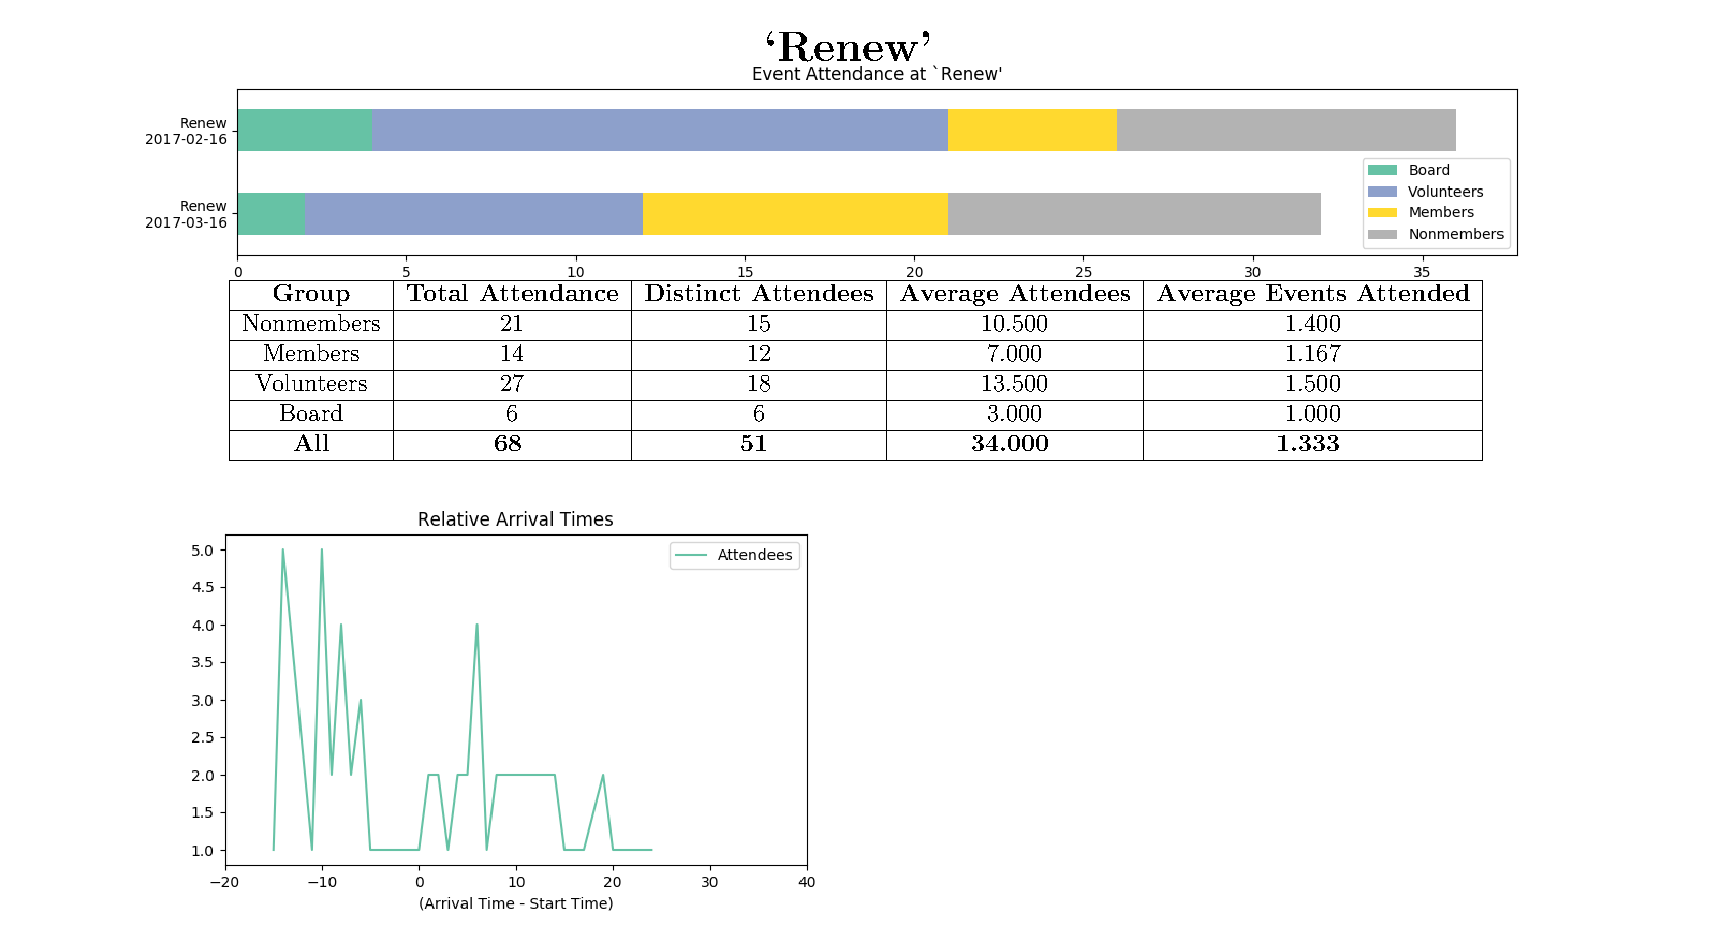
\includegraphics[width=5.3in]{./media/name.pdf}
\end{figure}
\pagebreak

Generate a report on all events named "Community Dinner" or "Freshmen Give Back Dinner"

\texttt{ \$ organ --names 'Community Dinner' 'Freshmen Give Back Dinner'}
\begin{figure}[H]
    \centering
    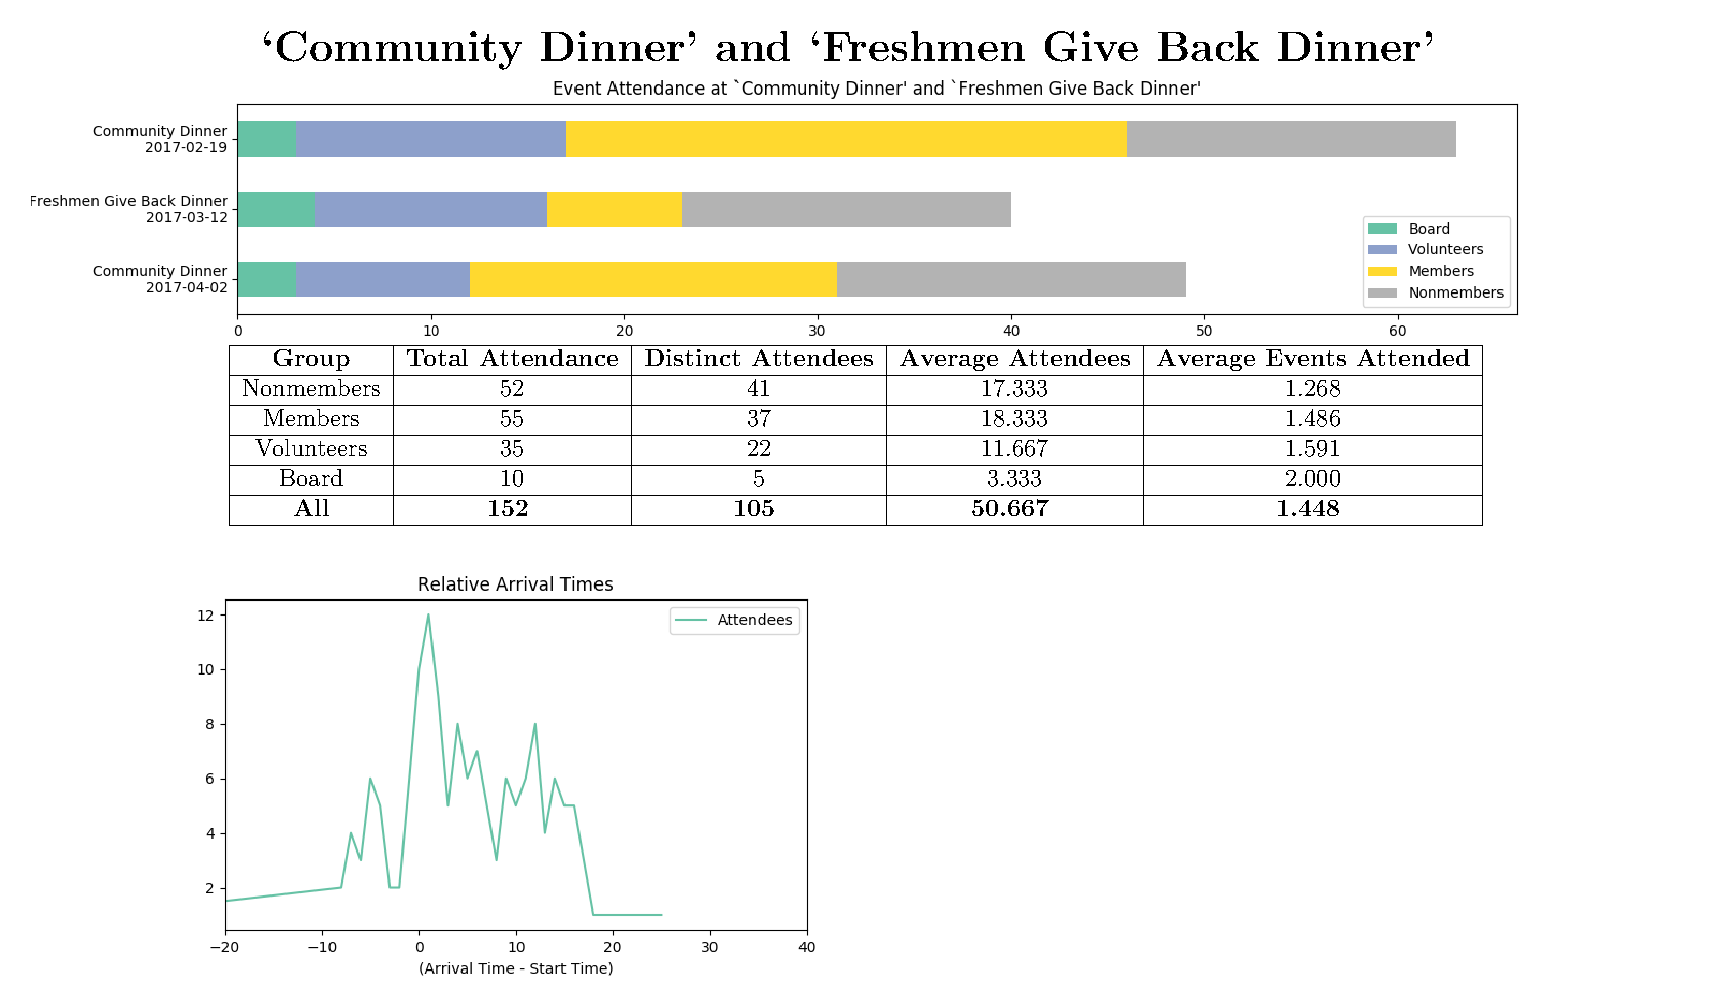
\includegraphics[width=5.3in]{./media/names.pdf}
\end{figure}
\pagebreak

Generate a report on all events on the Sundays of March:

\texttt{ \$ organ --dates 2017-03-05 2017-03-12 2017-03-19 2017-03-26}
\begin{figure}[H]
    \centering
    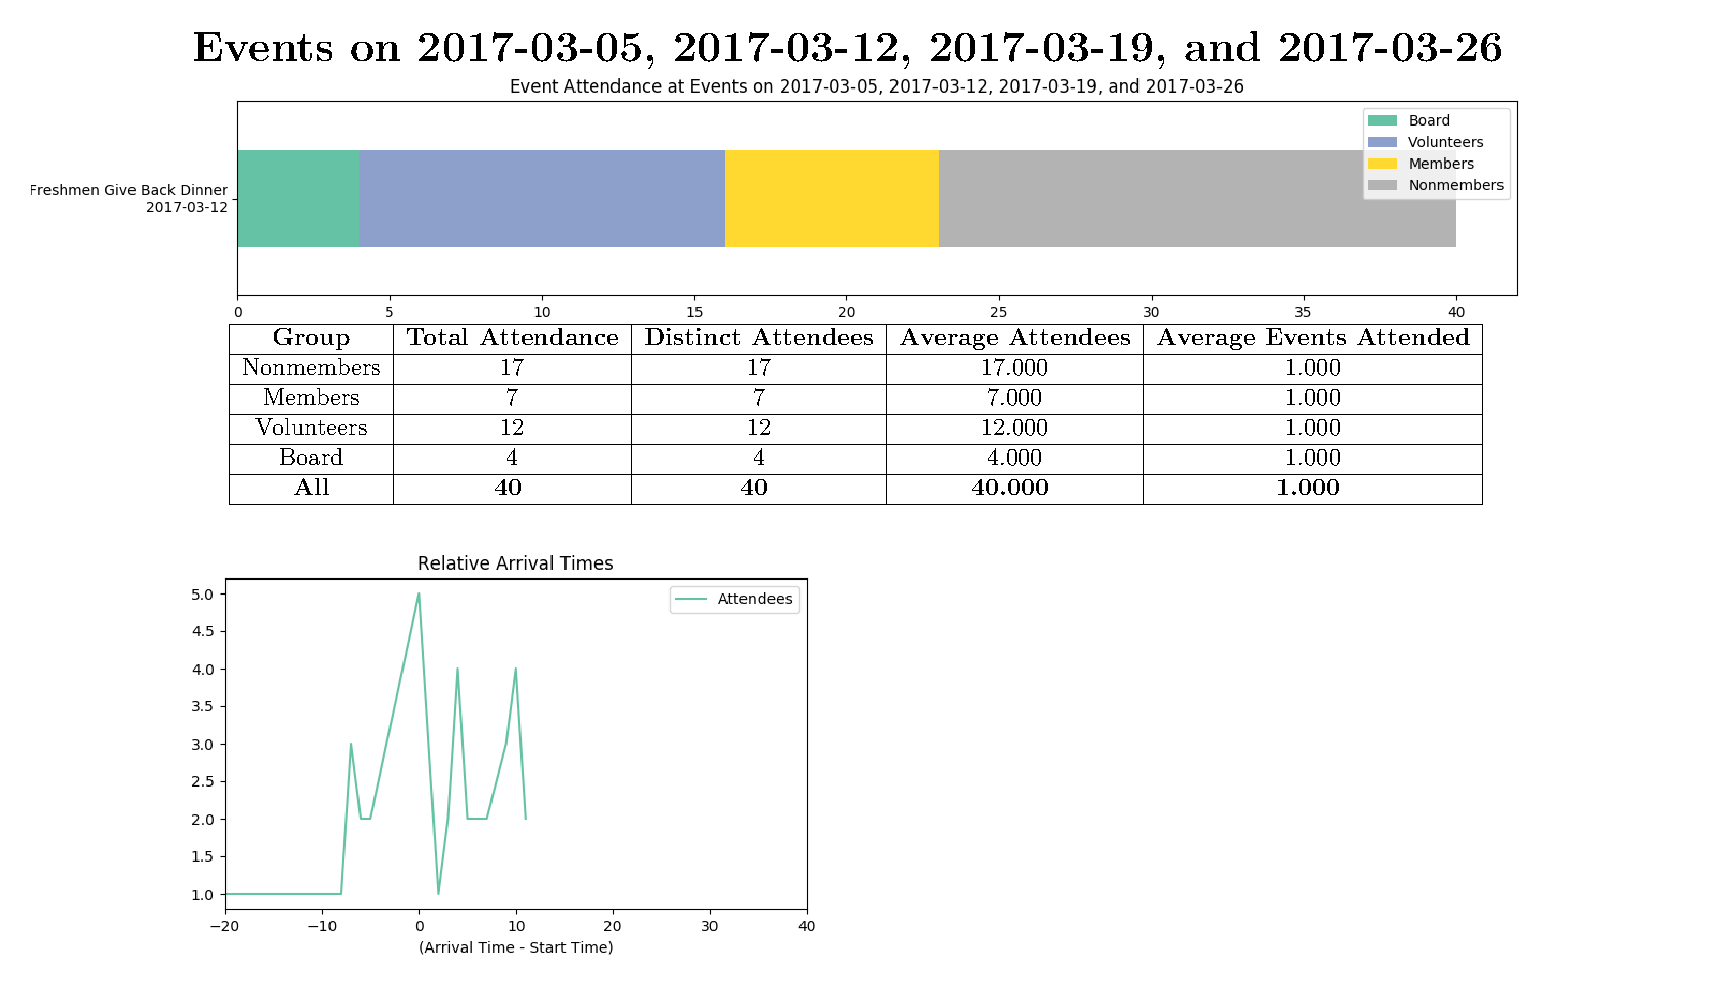
\includegraphics[width=5.3in]{./media/dates.pdf}
\end{figure}
\pagebreak

Generate a report on all events since March 15th:

\texttt{ \$ organ --start 2017-03-15}
\begin{figure}[H]
    \centering
    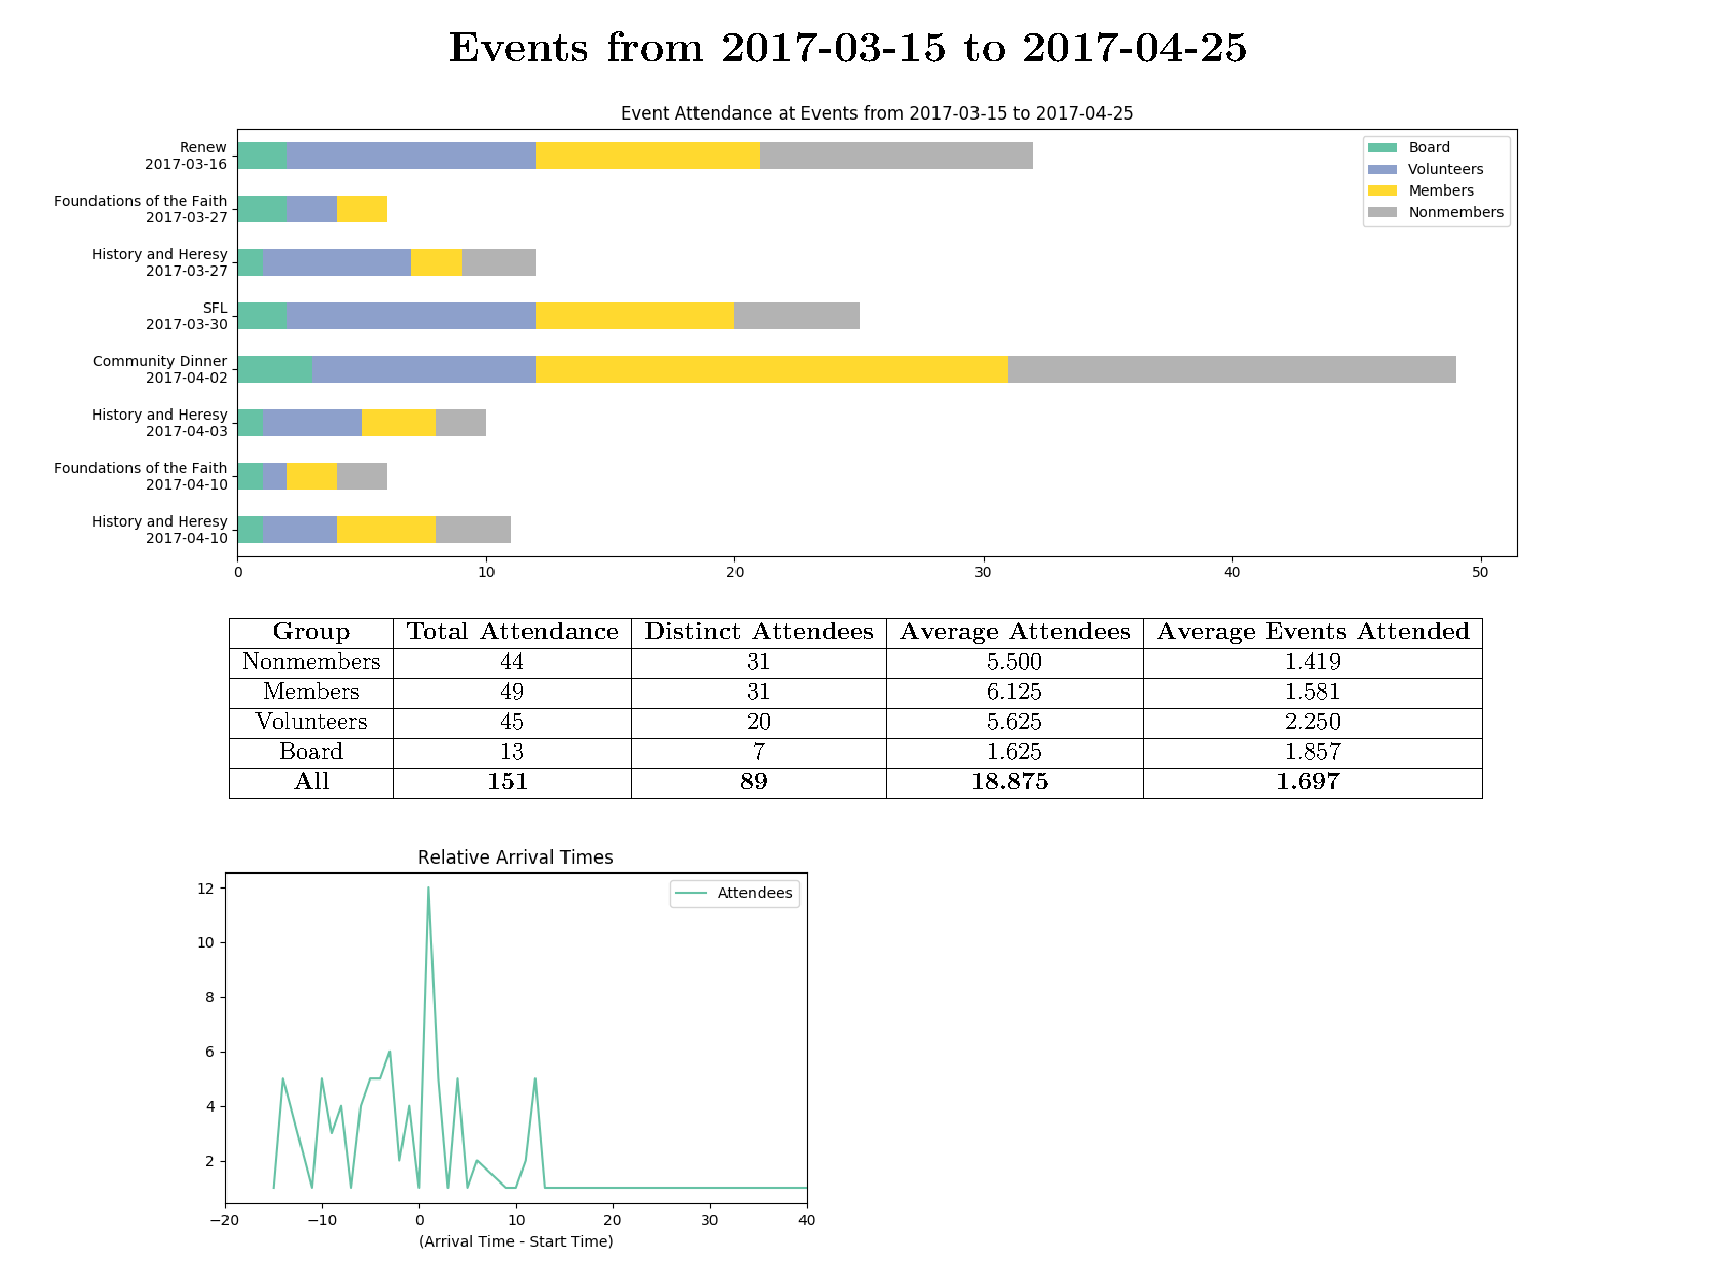
\includegraphics[width=5.3in]{./media/start.pdf}
\end{figure}
\pagebreak

Generate a report on all events between the start of the year and March 28th:

\texttt{ \$ organ --start 2017-01-01 --end 2017-03-28}
\begin{figure}[H]
    \centering
    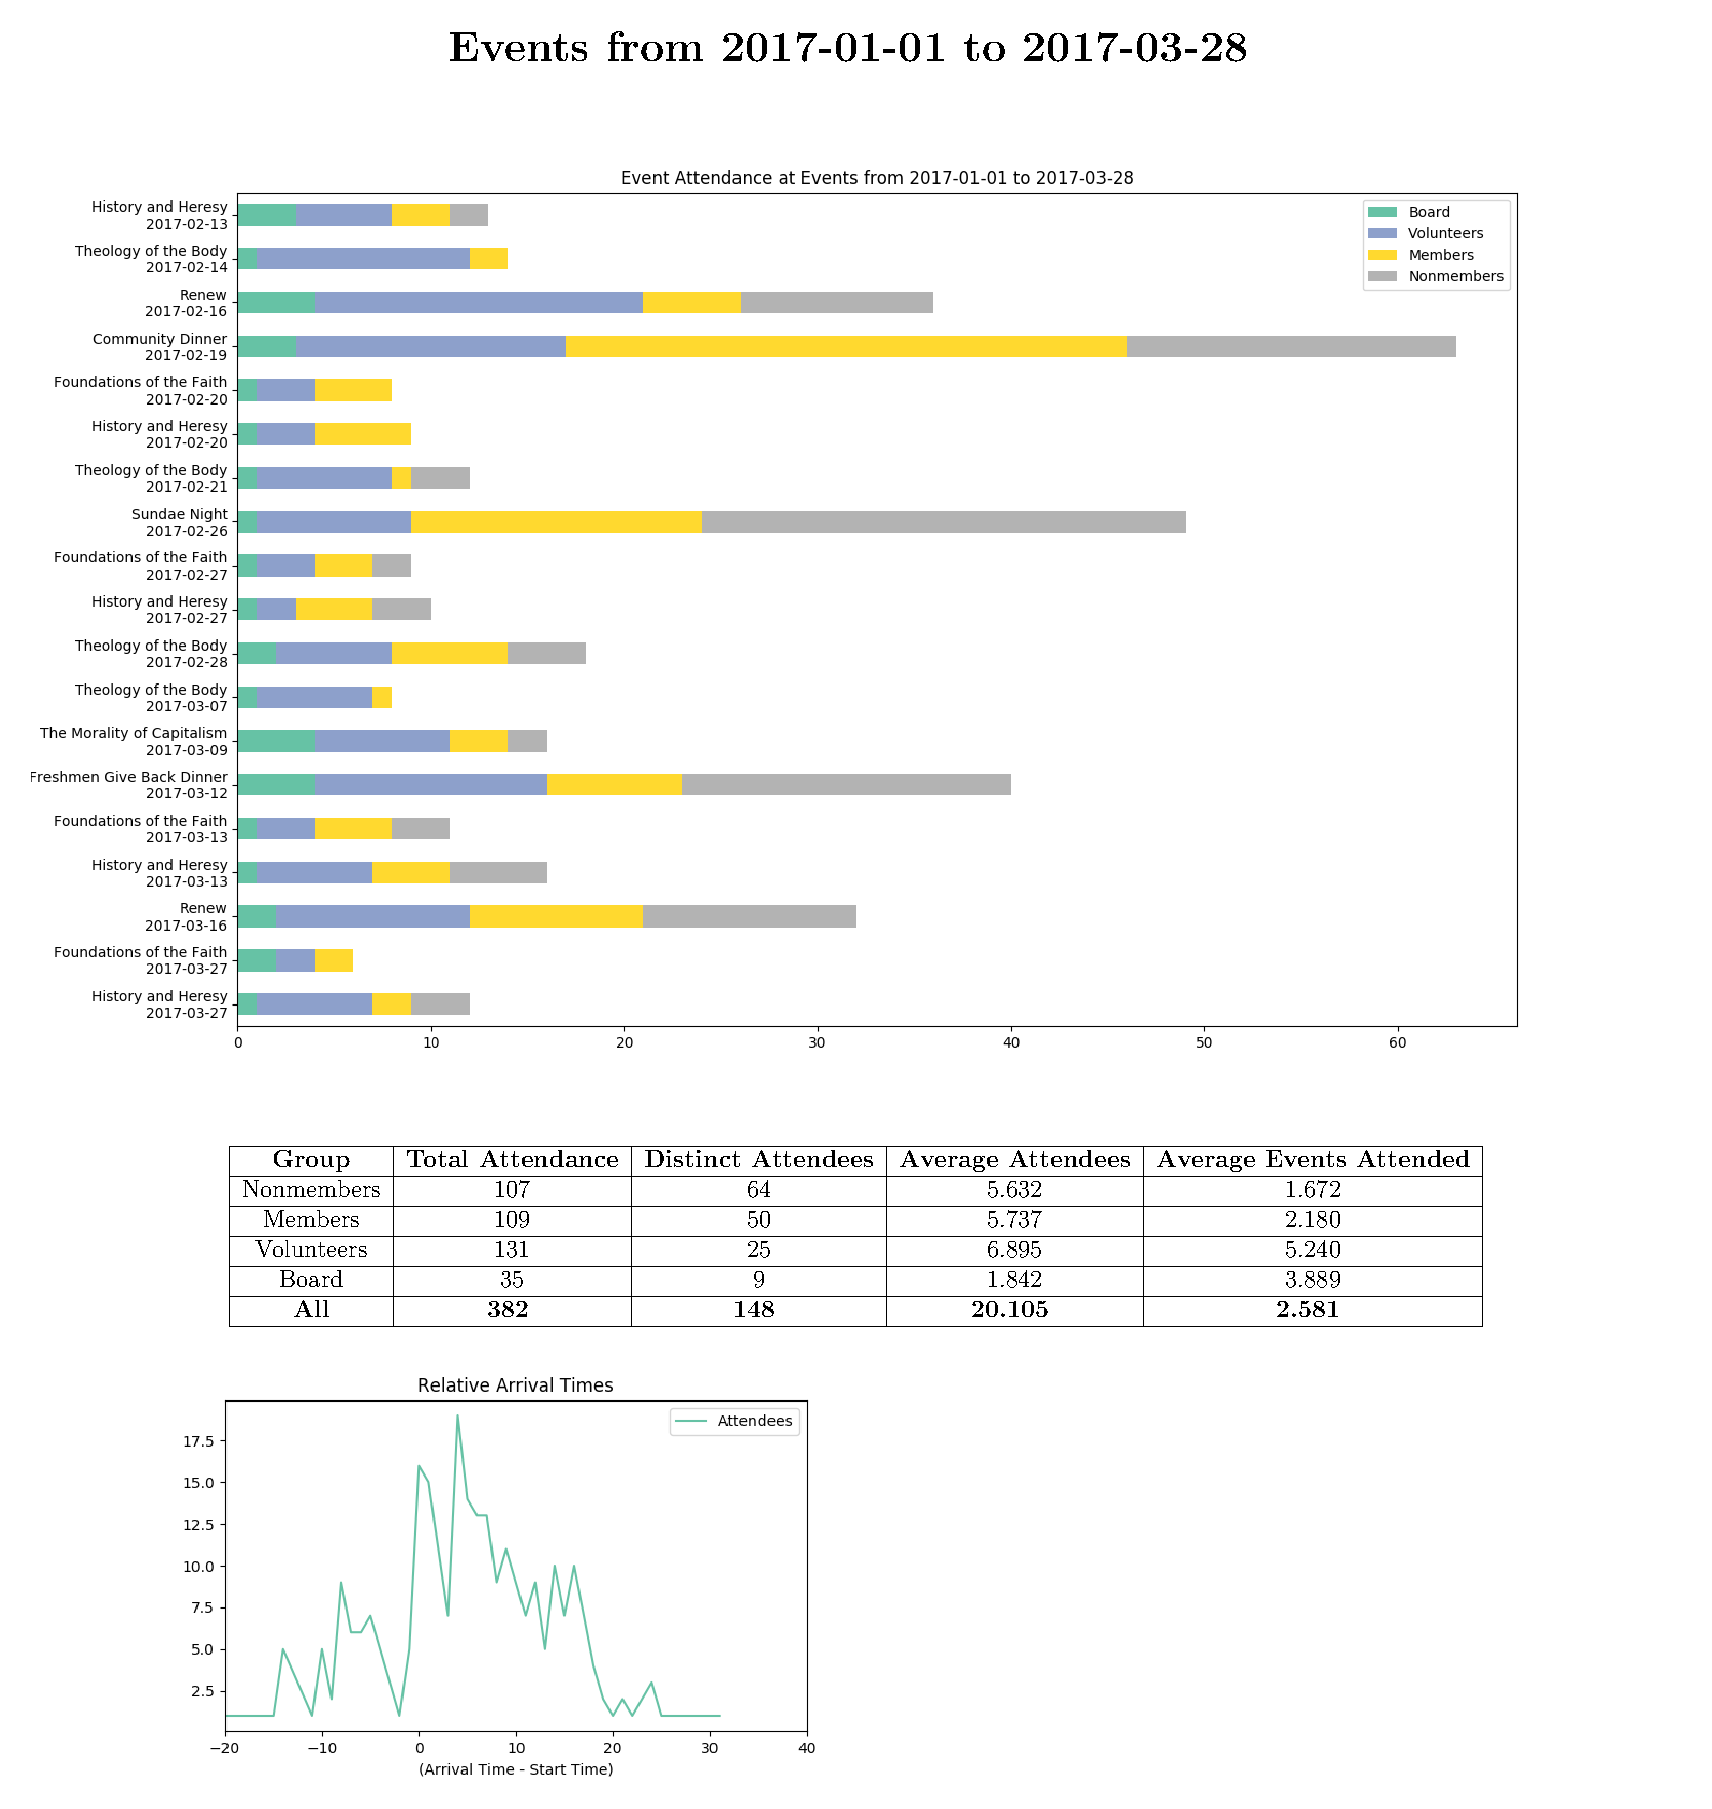
\includegraphics[width=5.3in]{./media/range.pdf}
\end{figure}
\pagebreak

Compare two groups of events by name:

\texttt{ \$ organ --names 'Foundations of the Faith' 'History and Heresy' vs 'Theology of the Body'}
\begin{figure}[H]
    \centering
    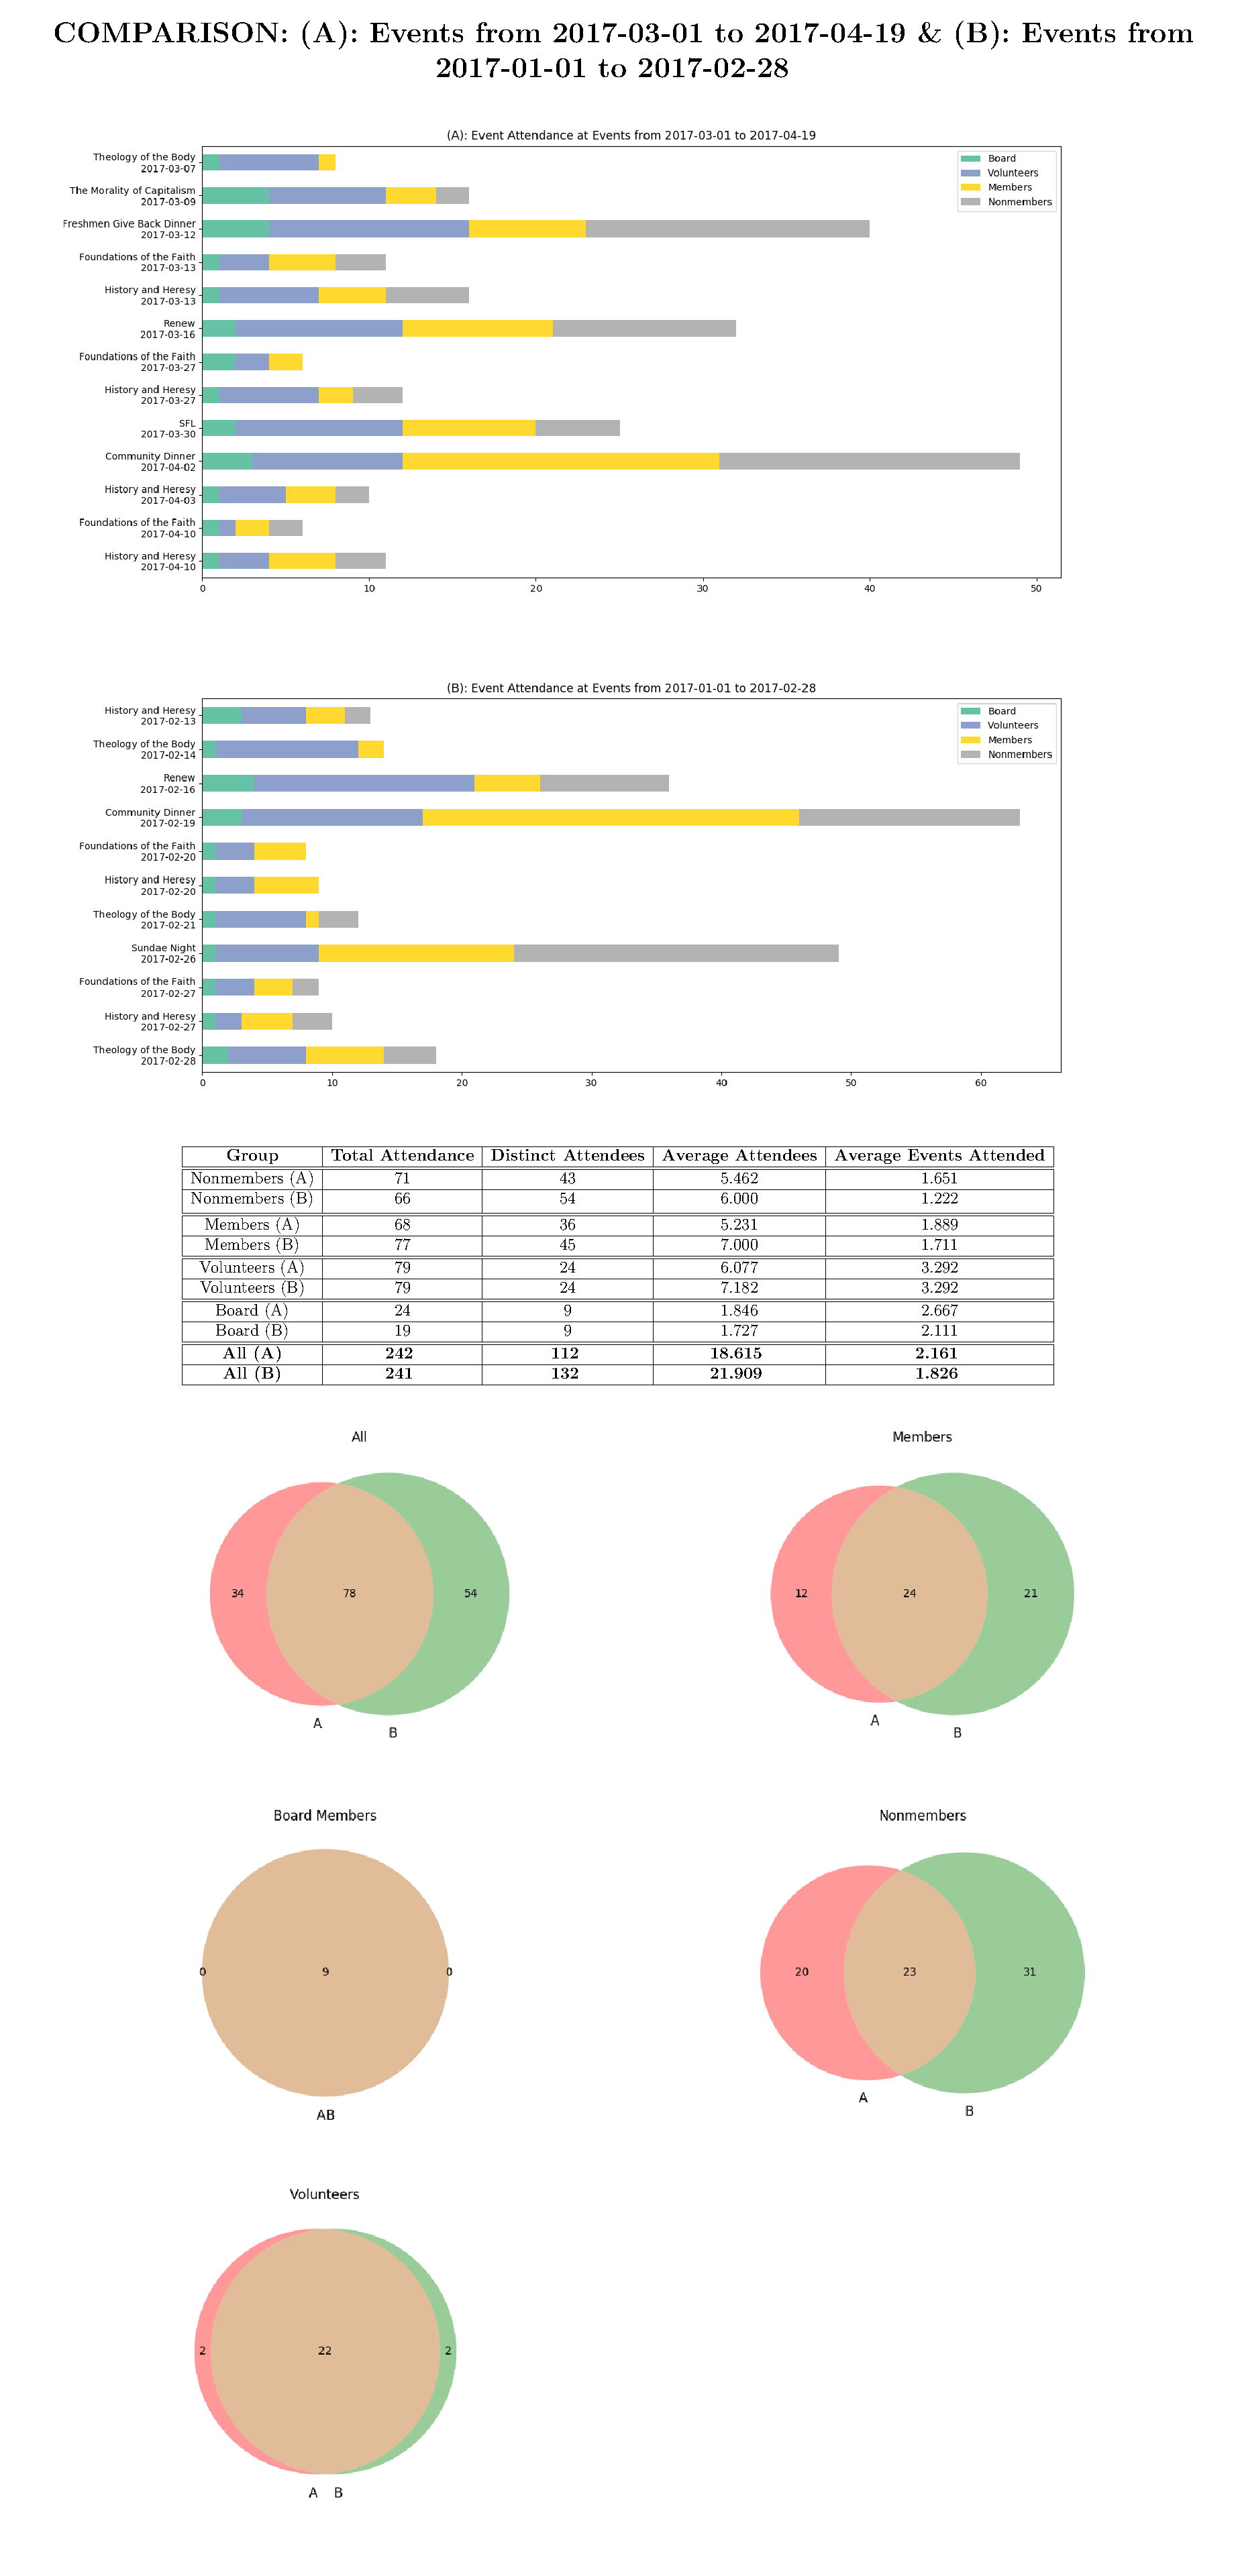
\includegraphics[width=3.5in]{./media/namescomp.pdf}
\end{figure}
\pagebreak

Compare the attendance of events in two time ranges:

\texttt{ \$ organ --start 2017-03-16 vs --start 2017-01-01 --end 2017-03-15}
\begin{figure}[H]
    \centering
    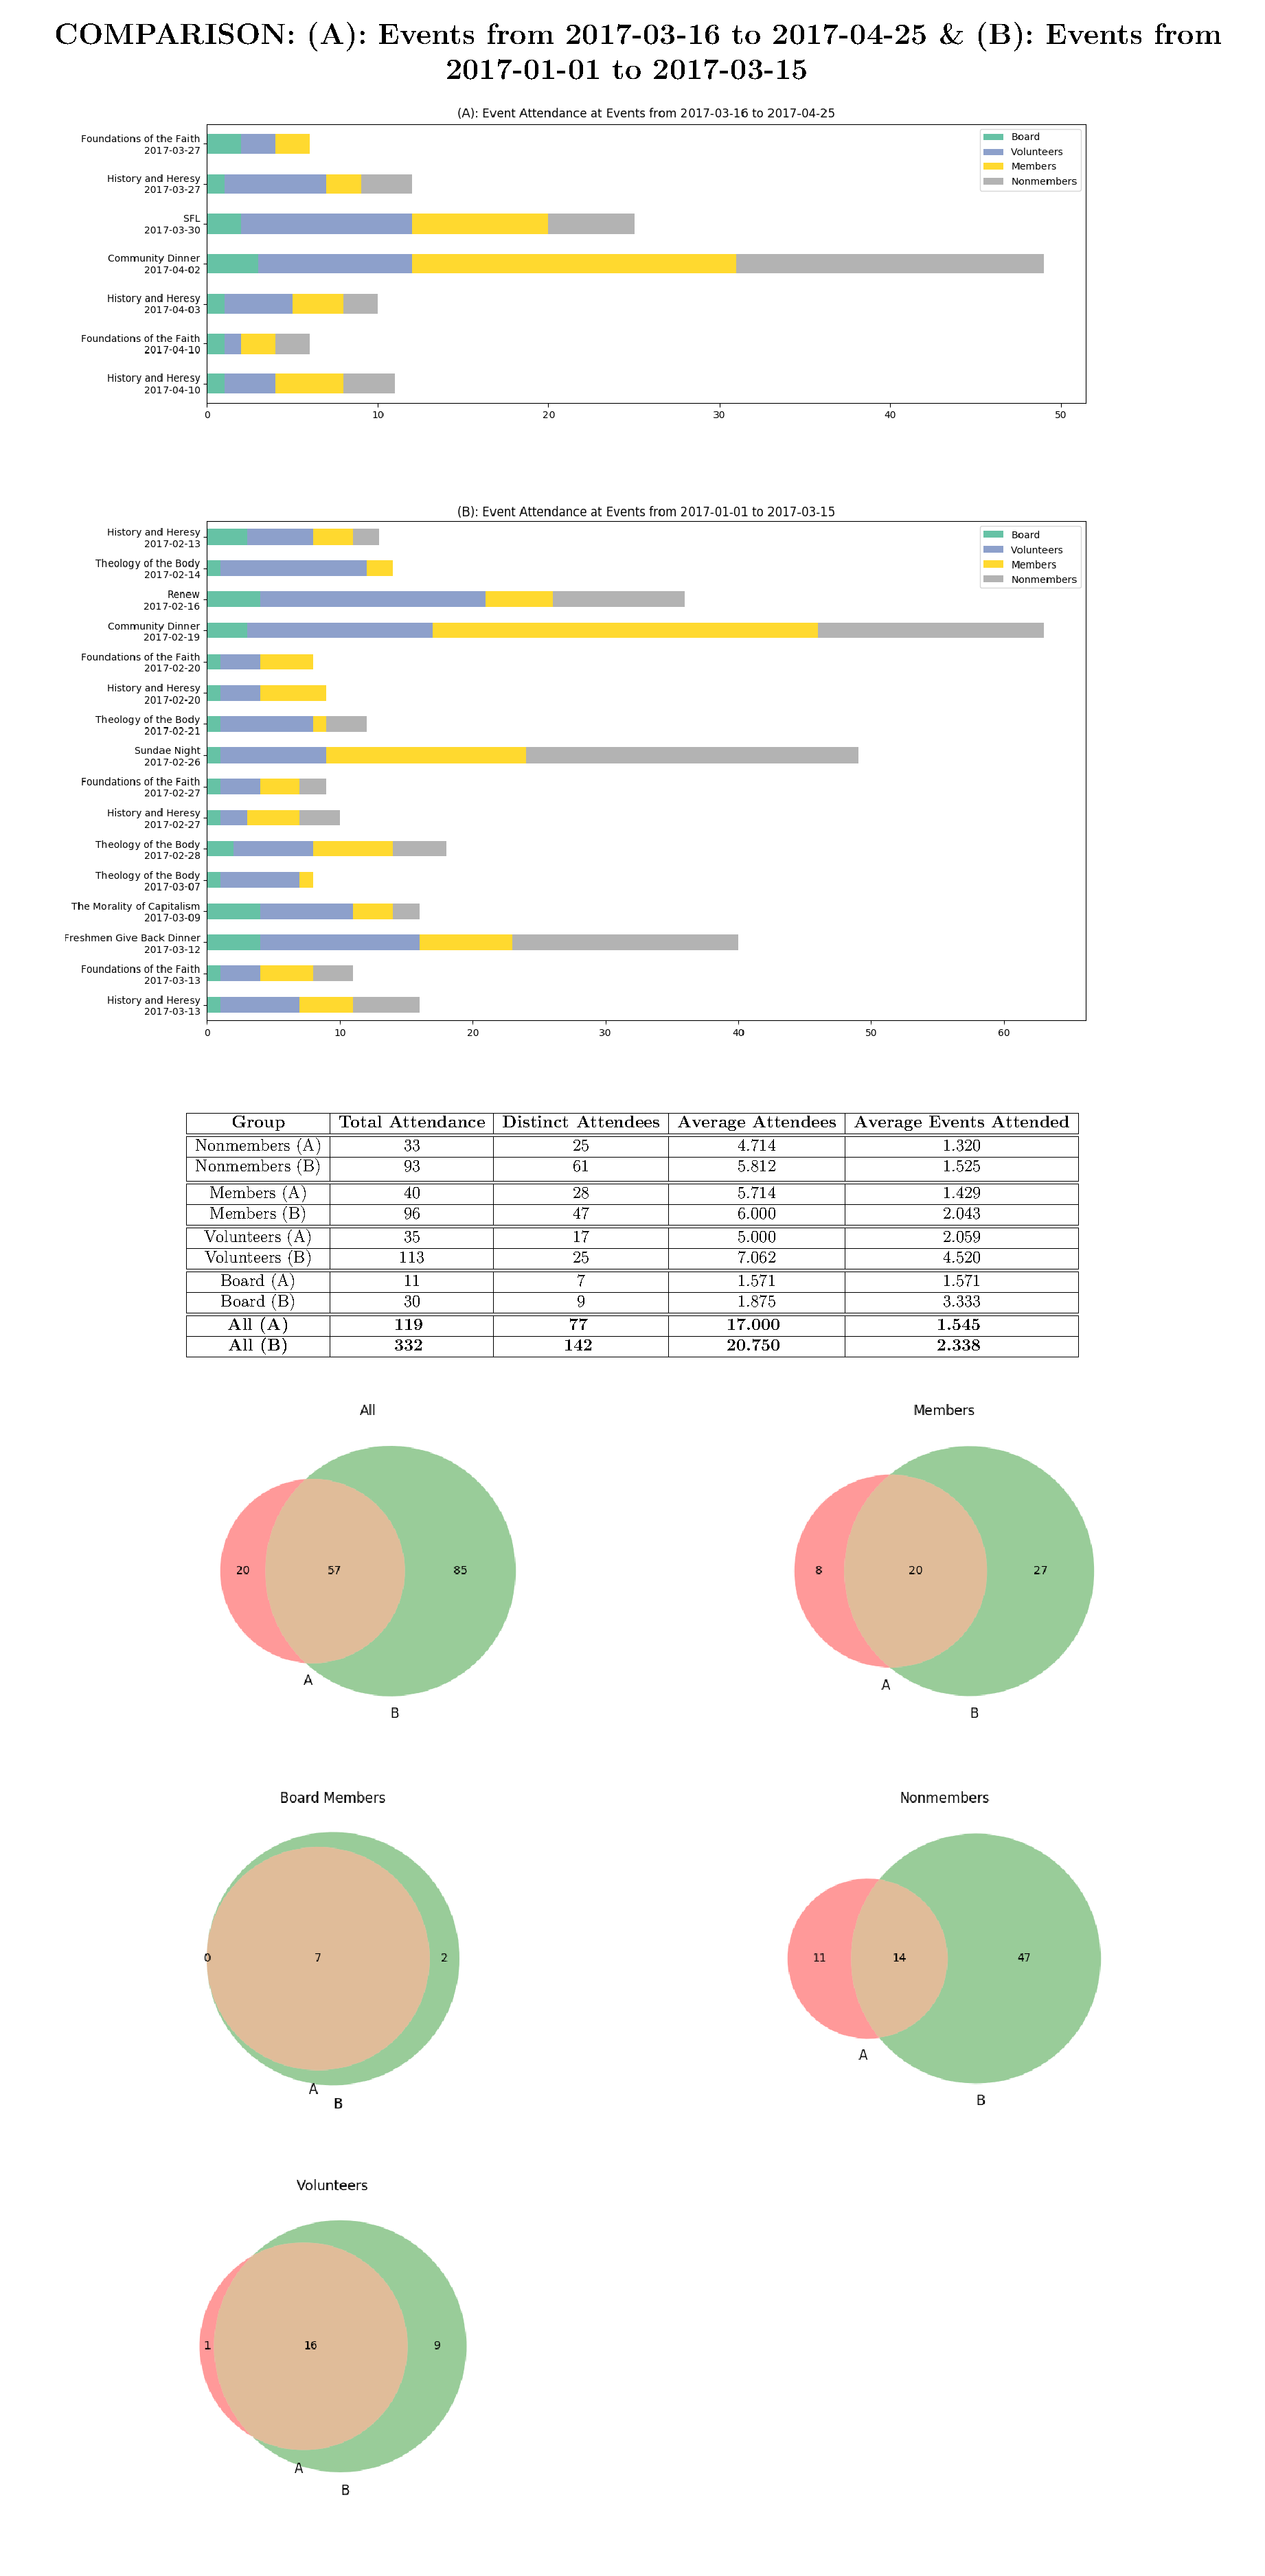
\includegraphics[width=4in]{./media/datescomp.pdf}
\end{figure}
\pagebreak

Compare attendance of a specific group of events across two ranges of time:

\texttt{ \$ organ --names 'Foundations of the Faith' 'History and Heresy' --start 2017-01-01 --end 2017-03-15 vs --names 'Foundations of the Faith' 'History and Heresy' --start 2017-03-16}
\begin{figure}[H]
    \centering
    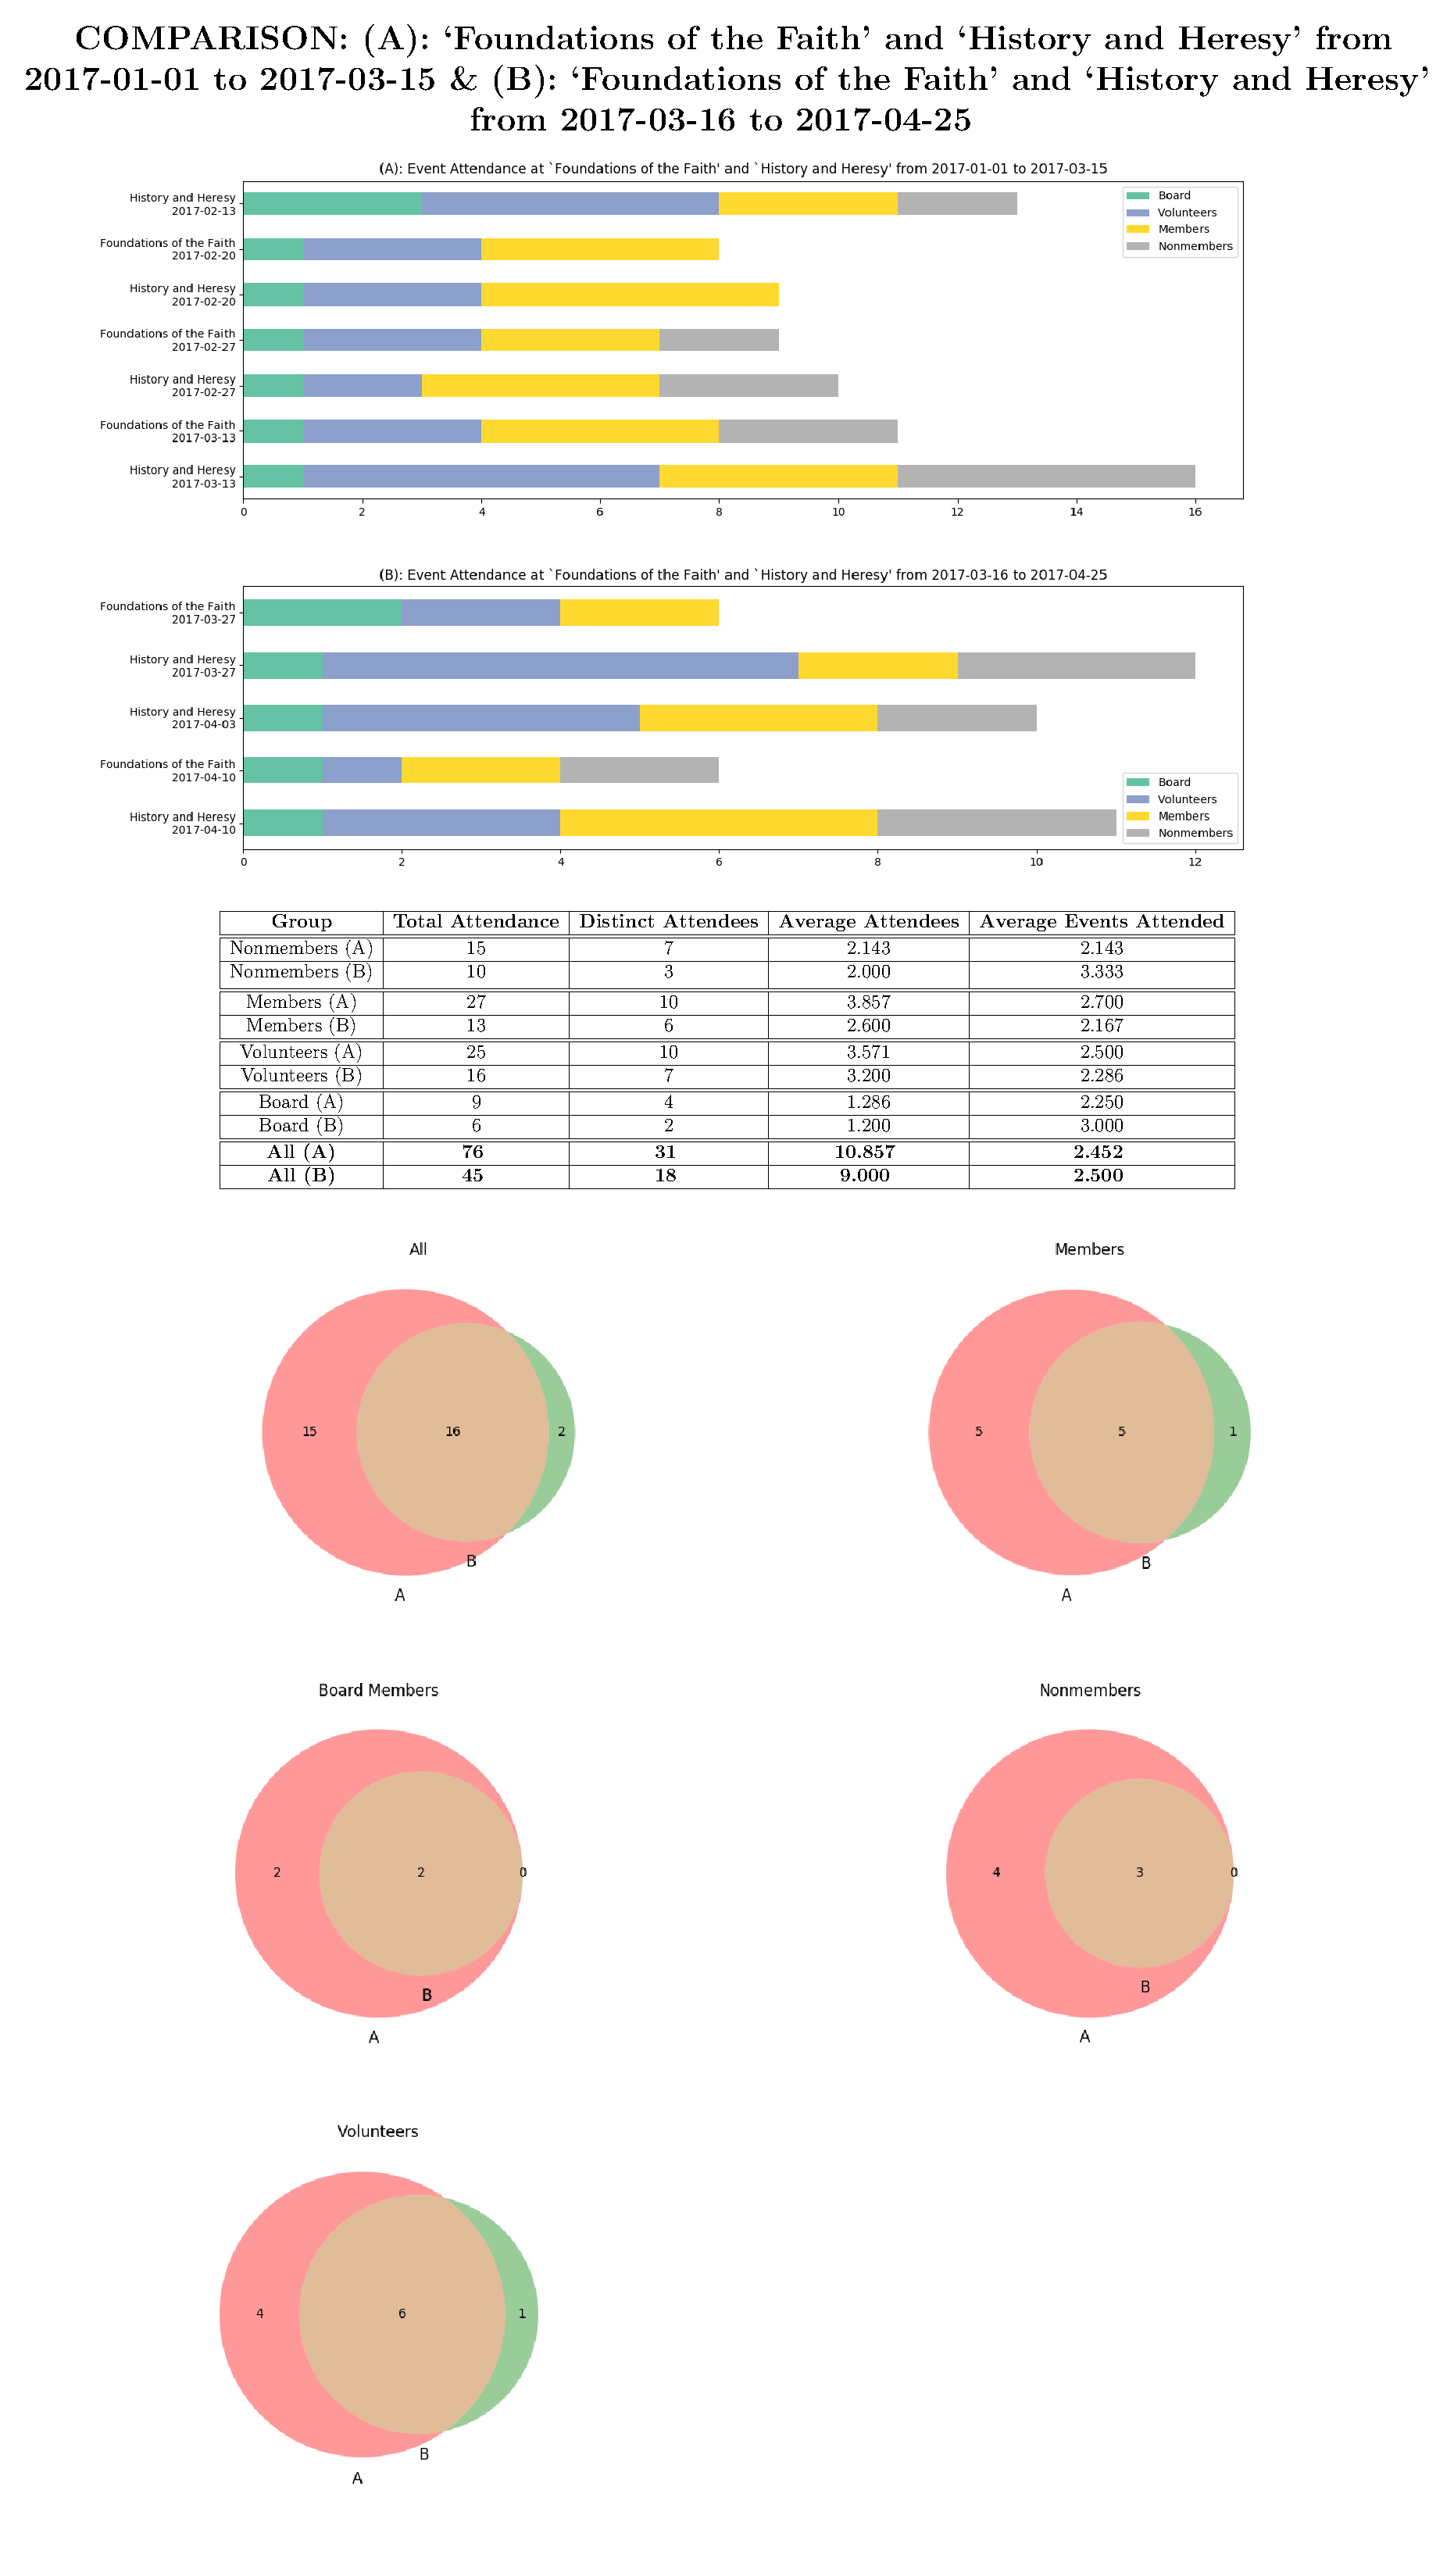
\includegraphics[width=4in]{./media/selfcomp.pdf}
\end{figure}
\pagebreak


\section*{Future Work}
The project as it stands has strong base functionality.
It is modular and extensible enough that new features can be slotted in without major headaches.
In the near future, I intend to extend functionality in several ways:

\begin{itemize}
    \item Replacing the current data-parsing-and-loading architecture with a module using the new OrgSync API upon its release
    \item Attendee-based reports: selecting groups of attendees to analyze and report on.
        This extends functionality beyond the current event-reporting model.
    \item Implementation of a graphical user interface
    \item Portability fixes, especially around handling of file paths
    \item Packaging through setup.py or Poet for easier installation
    \item Email list generation features
    \item Continued improvements to appearance of reports
\end{itemize}


\section*{Reflection}

This project did not go exactly in the direction I envisioned; the API issue, for one, was a serious speed bump.
Other changes came out of the design process --- this project included some big decisions, such as the shift towards report generation rather than a simple data display interface.
Making such changes was a particularly positive aspect of my experience working on the project; it was a great way to practice careful consideration of software design choices.

At a more technical level, this project has given me an initial grounding in data visualization.
The experience I built with the Pandas library is particularly valuable.
I've also reinforced my familiarity with relational databases, the implementation of command line interfaces, and python in general.

The strong dose of LaTeX in this project might not be the most marketable skill, but it has left me convinced of the utility of typesetting.
This old piece of technology has entrenched itself in my workflow since I started working with it for this project.
It's my new go-to for presentations, papers, and reports (yes, this one!).

I found that this  project was a rewarding learning experience overall.

\section*{Supporting Materials}
Alongside the submission of this final report, I have included a link to the source code of the project, a tarball of the data set used, and the presentation materials used for the in-office presentation.

% \printbibliography
\end{document}
